\chapter{RNN}

Transformer models represent a fundamental advancement in the processing of sequential data, offering a highly parallelizable and effective alternative to traditional sequence models. These models are composed of multiple layers of attention and feed-forward mechanisms, enabling them to capture both local and global dependencies within sequences. The overall structure of a transformer model is illustrated in Figure (ref). While transformers have found broad application in domains such as natural language processing, speech recognition, and computer vision, this work specifically focuses on their adaptation for biological sequence analysis.

To provide a structured introduction, this chapter begins with a review of recurrent neural networks (RNNs), which formed the basis for sequence-to-sequence learning via encoder–decoder frameworks. Their limitations, particularly in handling long-range dependencies, motivate the transition to attention-based architectures. Subsequently, the chapter presents a stepwise development of the transformer model, followed by an explanation on how this general framework can be modified to accommodate the unique properties of biological sequences.

In addition, the chapter outlines training methodologies designed to optimize performance in this domain, considering aspects such as regularization, data augmentation, and optimization strategies. Finally, the chapter concludes with a detailed examination of evaluation metrics relevant to transformer-based models, highlighting criteria necessary for assessing predictive accuracy, generalization, and biological interpretability.


\section{Recurrent Neural Network and Backpropagation}
Consider a dataset consisting of $N \in \mathbb{N}$ sequences. Each sequence $i \in \{1, 2, \dots, N\}$ contains $n \in \mathbb{N}$ observations, $x_i = \{x_{i,1}, x_{i,2}, \dots, x_{i,n}\}$, and $q \in \N$ response variables, $y_i = \{y_{i,1}, y_{i,2}, \dots, y_{i,q}\}$. Collectively, all observation and response sequences yield the matrices $X = \{x_1, x_2, \dots, x_N \} \in \R^{N \times n}$ and $Y= \{y_1, y_2, \dots, y_N \} \in \R^{N \times q}$, respectively. A recurrent neural network (RNN) processes such sequences using hidden states to produce estimates based on the current and previous inputs, see Figure \ref{fig:example RNN}. The hidden state at each observation is defined recursively as
\begin{align*}
    h_{n} = f_\theta(h_{n-1}, x_n),
\end{align*}
where $h_n \in \R^p$ denotes the hidden state at observation $n$. The function $f_\theta : \R^{p} \times \R^N \to \R^{p}$ is an observation-invariant activation function parameterized by $\theta = \{ W, U, b_h\}$, where $W \in \R^{p\times p}$ is an invariant weight matrix between the hidden states, $U \in \R^{p \times N}$ is an invariant weight matrix between the inputs and the state, and $b_h \in \R^p$ is the bias between the states. Generally, the activation function used, is the hyperbolic tangent, at each entry of the vector. Thus, the hidden state at each observation can be described as
\begin{align*}
    h_n = \tanh(Wh_{n-1} + UX_{n-1} + b_h).
\end{align*}
Since $\tanh: \R \to (-1, 1)$, the resulting hidden state for the $n$'th observation $h_n \in (-1, 1)^p$. From each of the hidden states, an estimate can be obtained
\begin{align*}
    \hat{y}_n = g_\Theta(h_n),
\end{align*}
where $g_\Theta :\R^p \to \R^q$ is an invariant activation function parameterized by $\Theta = \{V, b_y\}$. Here $V \in \R^{q \times p}$ is a weight matrix between the hidden state and the output, and $b_y \in \R^q$ is a bias term. To represent the output as a probability distribution, the activation function, $g_\Theta (\cdot)$, is typically chosen to be the softmax function, yielding
\begin{align*}
    \hat{y}_{n,j} = \text{softmax}\left(Vh_n + b_y\right)= \frac{\exp((Vh_{n} + b_y)_j)}{\sum^q_{k=1}\exp((Vh_{n} + b_y)_k)},
\end{align*}
where $\hat{y}_{n,j}$ denotes the probability assigned to the j-th entry of the n-th input in the sequence. 
\begin{figure}
    \centering
    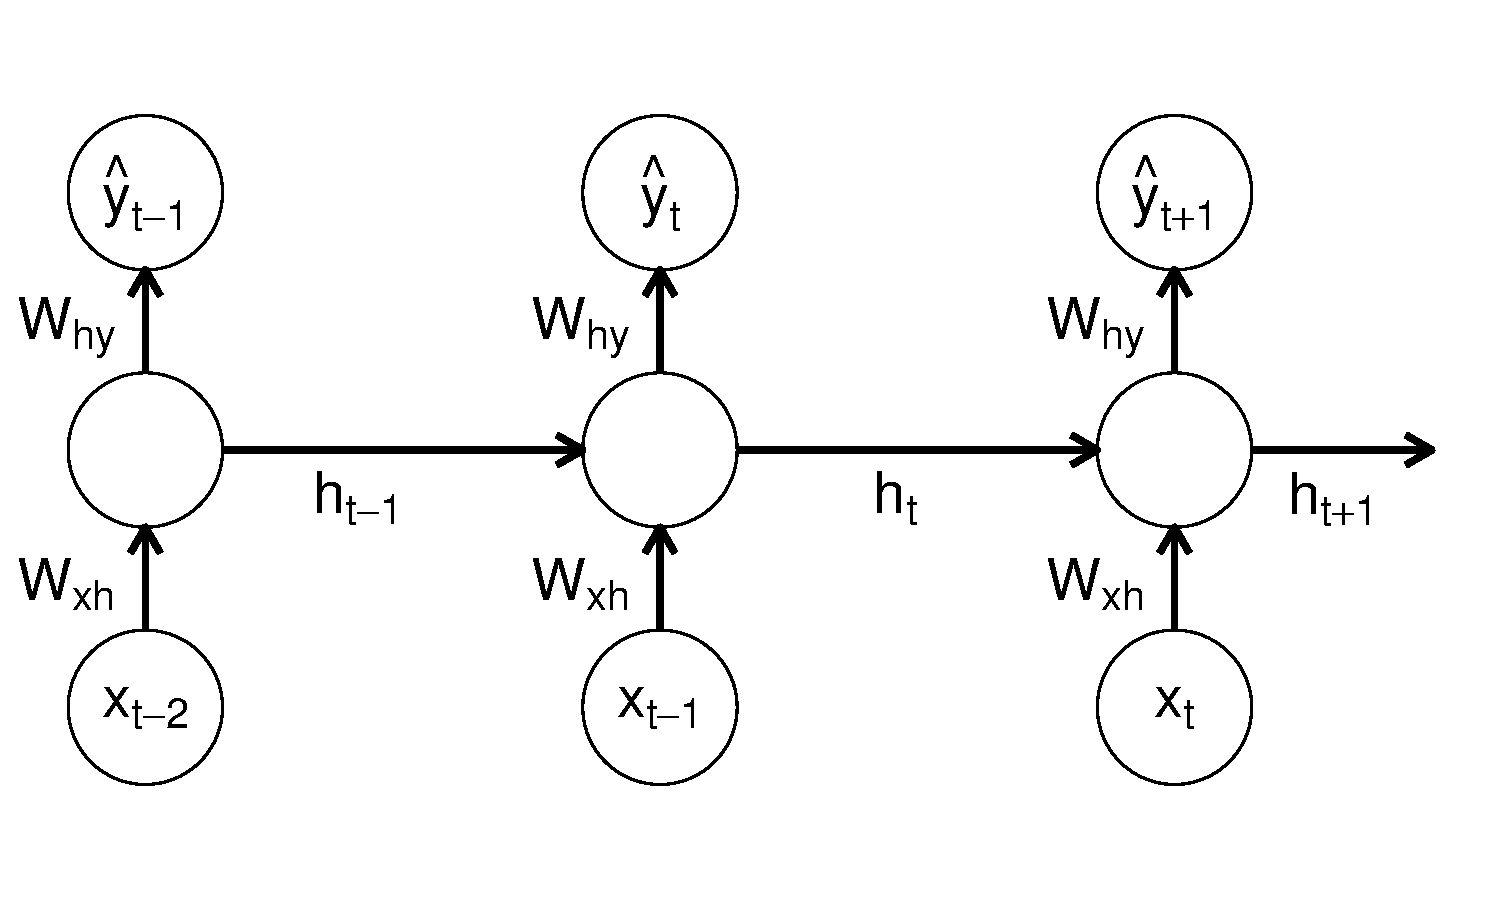
\includegraphics[width=0.8\linewidth]{fig/img/RNN/RNN_Example.pdf}
    \caption{Example of an RNN}
    \label{fig:example RNN}
\end{figure}

